\documentclass[11pt, a4paper]{article}

\usepackage[utf8]{inputenc}
\usepackage{graphicx}
\graphicspath{ {images/} }
\usepackage{mathtools}
\usepackage{amssymb}
\usepackage{amsmath}
\usepackage[ngerman,english]{babel}
\usepackage{cite}
\usepackage{bibgerm}
\usepackage{fullpage}
\usepackage[top=1.5cm,bottom=1.5cm,left=3.5cm,right=2.5cm,headsep=1.5cm,includeheadfoot]{geometry}
\usepackage{tabularx}
\usepackage{caption}
\usepackage{subcaption}
\usepackage{eurosym}
\usepackage{enumitem}
\usepackage{multicol}
\usepackage{tikz}
\usepackage{tkz-euclide}
\usepackage{pgfplots}
\usepackage{pdflscape}
\usepackage{acronym}
\usepackage{blindtext}
\usepackage{ifthen}
\usepackage{setspace}
\usepackage{cancel}
\usepackage{color}
\usepackage{listings}
\usepackage{comment}
\usepackage{xcolor}
\usepackage{colortbl}
\usepackage[parfill]{parskip}
\usepackage{url}

\usepackage{fancyhdr}
\pagestyle{fancy}

\fancyhf{} % clear all
\fancyhead[L]{\leftmark}
\fancyfoot[C]{-- \thepage{} --}
%\setlength{\headheight}{15pt}
\renewcommand{\headrulewidth}{0.5pt}
\renewcommand{\footrulewidth}{0pt}
\setlength{\skip\footins}{0.7cm}

\usetikzlibrary{graphs}
\usetikzlibrary{positioning}

\onehalfspacing
\setlength\parindent{0pt}

%\everymath{\displaystyle}

\allowdisplaybreaks

\definecolor{AI-BLUE}{rgb}{0,0.57,0.87}

% Eigene Befehle
\newcommand\q[1]{\glqq{}#1\grqq{}}
\renewcommand\equiv{\Leftrightarrow}
\newcommand\vertequal[2]{\underset{\underset{#2}{\parallel}}{#1}}
\newcommand\cif{\text{if }}
\newcommand\abs[1]{\left|#1\right|}
\newcommand\norm[1]{\abs{\abs{#1}}}
\newcommand\diff[1]{\text{ d#1}}
\newcommand\av[1]{\left\langle#1\right\rangle}
\newcommand\ev[1]{\mathbb{E}\left(#1\right)}
\newcommand\br[1]{\left(#1\right)}
\newcommand\ubr[2]{\underbrace{#1}_{#2}}
\newcommand\quer[1]{\overline{#1}}
\newcommand\setequal{\overset{!}{=}}
\newcommand\dint{\displaystyle \int}
\newcommand\dsum{\displaystyle \sum}
\newcommand\dprod{\displaystyle \prod}
\newcommand\closedInt[2]{\left[#1,#2\right]}
\newcommand{\checkbox}{\Large \Square \normalsize \hspace{0.4cm}}

\newcommand\myref[1]{\ref{#1} (S. \pageref{#1})}
\newcommand\myrefcomma[1]{\ref{#1}, S. \pageref{#1}}

\begin{document}

\thispagestyle{empty}

\setlength{\hoffset}{-0.5cm} % center title page

\lstset{
  basicstyle=\small,           % the size of the fonts that are used for the code
  breaklines=true,             % sets automatic line breaking
  captionpos=b,                % sets the caption-position to bottom
  frame=single,                % adds a frame around the code
  keepspaces=true,             % keeps spaces in text, useful for keeping indentation of code (possibly needs columns=flexible)
  numbers=right,               % where to put the line-numbers; possible values are (none, left, right)
  showspaces=false,            % show spaces everywhere adding particular underscores; it overrides 'showstringspaces'
  stepnumber=1,                % the step between two line-numbers. If it's 1, each line will be numbered
  tabsize=4,                   % sets default tabsize to 4 spaces
  xleftmargin=0.14cm		   % sets left margin
}


\begin{titlepage}
    \begin{center}
    \vphantom{0cm}
    \LARGE \textbf{Report}\\
    \vspace{3cm}
    \normalsize
    Study Project Documentation \\
    in the Master Program of \textcolor{AI-BLUE}{[Applied Computerscience]}\\
    at the Ruhr-University Bochum\\
    in the Winter Term 2015/16\\
    \vspace{4cm}
    \huge \textbf{Convolutional Neural Networks} \\
    \vspace{4cm}
    \normalsize
    \textbf{Project Participants}\\
    B. Sc. Christian Andreas Mielers (108 011 204 956)\\
    B. Sc. Phil Yannick Schrör (108 011 214 024)\\
    \vspace{2cm}
    \textbf{Project Supervisor:}\\
    PD Dr. Rolf P. Würtz
    \end{center}
\end{titlepage}

\newpage
\pagenumbering{arabic}
\setcounter{page}{2}

\tableofcontents

\newpage
\section{Introduction}
Convolutional neural networks (CNNs) are powerful tools in the field of machine learning. Their strength results from the efficient use of free parameters by exploiting the spatial structure of their input. Instead of learning every weight in the INPUT $\times$ OUTPUT matrix of a fully connected layer, a convolutional layer learns the weights in filters of a fixed size. Since the filters are generally tiny compared to a full weight matrix, using many filters and layers becomes feasible. The convolution operation with those filters then produces a layer response that indicates the local features represented by the filters.

To reduce the amount of data passed through the network, pooling layers that combine the values in small regions of the input into a single value can be used. One can then think of the consecutive application of convolutional and pooling layers as mechanisms to iteratively integrate features from ever more remote locations of the image into a compact representation. Fully connected layers can the be used on the representations learned by these layers to perform classification of the input.

Since images typically contain a lot of spatial structure, they are well suited for processing by such a CNN. To study and evaluate the properties of CNNs, we considered a network layout described in \cite{multi-column-neural-network-gtsrb}. Multiple networks which consist of three pairs of convolutional and pooling layers followed up with two fully connected layers were combined into a committee to solve the GTSRB challenge described in \cite{gtsrb}. We used the layout of one such network on the GTSRB dataset and two other datasets and measured the resulting accuracy. The filters on the various convolutional layers were visualized. We also transfered the filters learned on the gtsrb dataset to the other datasets and only trained the fully connected layers to evaluate how well they generalize.

\section{Network details}

\section{Experiments with GTSRB}
The GTSRB dataset described in \cite{gtsrb} is a collection of $39209$ images in a training set and $12630$ images in a test set. In total, there are $43$ classes. The images were taken while driving through german streets and cropped to only contain the traffic sign and some boundary around it. For each physical traffic sign there are many images that vary in distance, angle and occlusion since they were taken while the car passes them. For each image, annotations exist that locate the bounding box of the traffic sign. To generate fixed-size images for our network, we extracted only that part given by the bounding box and rescaled it to $48\times48$ pixels. As an additional preprocessing step, contrast normalization was applied to reduce the considerable illumination differences present in the images.
% Morphen vs. nicht morphen
% Relu

\section{Filter reuse}

In order to examine how well the convolution filters trained on the GTSRB dataset generalize, we used the GTSRB filters also on other datasets. After several epochs of training on the GTSRB data, we copied the weights to another CNN and continued the training of the fully connected layers in the other model. The weights of the convolutional layers, i.e. the filters, remained unchanged. To find out, how well this approch works in terms of training time and classification results, we also trained completely new weights on these comparison datasets.

\subsection{COIL100 dataset}

The first dataset we used is the COIL100 dataset (Columbia Object Image Library) \cite{columbia_object_image_library}, which contains images of 100 different objects. The objects were placed on a black turntable in front of a black background. 
\begin{figure}[h!]
	\centering
	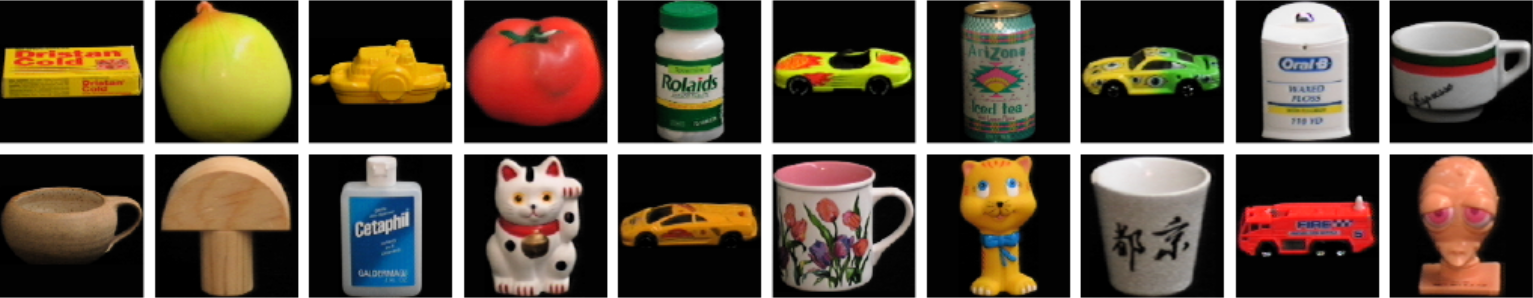
\includegraphics[width=1\textwidth]{coil100}
	\caption{A subset of 20 objects taken from the COIL100 dataset.}
	\label{fig:coil100_objects}
\end{figure}
In order to be able to present the learning algorithm many different views on one single object, the camera took a photo of the rotating object, each time it has turned by 5 degrees.

\begin{figure}[h!]
	\centering
	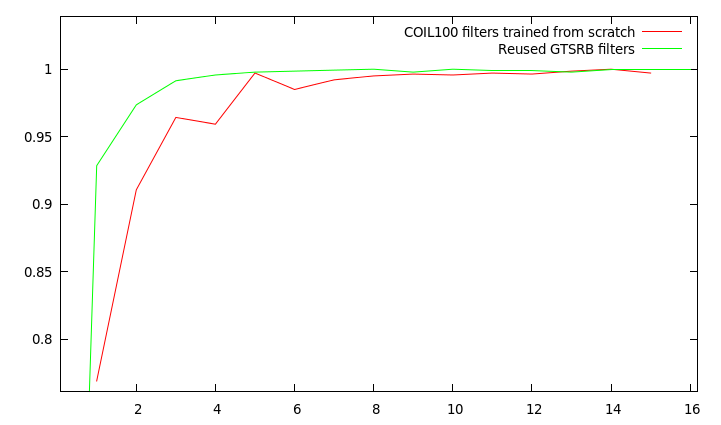
\includegraphics[width=1\textwidth]{coil100_results.png}
	\caption{Results on the COIL100 dataset with filters completely trained from scratch and with reused GTSRB filters.}
	\label{fig:coil100_results}
\end{figure}



\subsection{INRIA dataset}

After achieving excellent results on the COIL100 dataset, we tried to get similar results on a probably more difficult dataset. The dataset we chose is the Head Pose Image Database \cite{estimating-face-orientation-inria} from the French Institute for Research in Computer Science and Automation (INRIA). The dataset consists of 15 persons, two series per person and 93 JPEG-images per series. In each series the depicted person changes its head posture gradually. One of the two series shows the person with a certain feature like glasses, the other series does not. Figure \ref{fig:inria_different_angles} shows some example images for one person taken from one series.

\begin{figure}[h!]
	\centering
	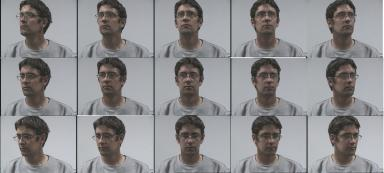
\includegraphics[width=0.8\textwidth]{inria_different_angles}
	\caption{Person 12 presented from different angles.}
	\label{fig:inria_different_angles}
\end{figure}

The problem appears to be harder than the COIL100 problem, because the persons in the INRIA dataset are more similar to each other than the objects in the other dataset.

\begin{appendix}
	\section{Implementation}
	\section{Visualization}
\end{appendix}

\addcontentsline{toc}{section}{References}
\bibliography{ref}{}
\bibliographystyle{alpha}

\end{document}






